\section{Experimental Results}

\subsection{Experimental Settings}
We use our curated cardiac arrest cohort from CHOA-CICU to conduct 5-fold cross-validation. We further ensure that no patient appears in both the training and testing sets for an unbiased evaluation.
As defined in Sec.~\ref{sec:study}, our research problem, early risk prediction of CA, is formulated asa a binary classification task. Accordingly, we employ a broad set of binary classification metrics, including balanced accuracy (Bal\_Acc), F1 score, Matthews Correlation Coefficient (MCC), Area Under the Precision-Recall Curve (AUPRC), and Area Under the Receiver Operating Characteristic Curve (AUROC), to comprehensively assess model performance while accounting for the inherent class imbalance (admission-wise CA incidence $=3.1\%$). 
% talk about the metrics a bit
In our evaluation, CA events are treated as the positive class. 
Among these metrics, Bal\_Acc is a specifically designed metric to avoid inflated performance on imbalanced dataset, which is essentially arithmetic mean of sensitivity and specificity in binary classification case. F1 is a harmonic mean of the precision and recall. 
MCC is defined as
\begin{equation}
    \text{MCC}=\frac{tp\times tn - fp \times fn}{\sqrt{(tp+fp)(tp+fn)(tn+fp)(tn+fn)}},
\end{equation}
where is generally regarded as a balanced metric for imbalanced case. A MCC of $+1$ presents a perfect prediction, $0$ an random prediction, and $-1$ an inverse prediction. AUROC and AUPRC both assess trade-offs between key performance rates. While AUROC is widely used—providing a threshold-independent evaluation of the balance between TPR and FPR and serving as a valuable benchmark for comparison with prior work—AUPRC is often more informative in scenarios with class imbalance~\cite{tomavsev2021use}, as it emphasizes the trade-off between precision and recall and focuses on performance for the minority (positive) class.

\begin{table*}[ht!]
\centering
\centering
\caption{Experimental results on CHOA-CICU curated cohort (numbers in percentage).}
\label{tab:CHOA_main_exp}
\begin{tabular}{c|ccccc}
\toprule
Model & Bal\_Acc & F1 & MCC & AUPRC &AUROC\\
\multicolumn{6}{c}{\textit{Clinician Derived Risk Scores}} \\
KNN-Dtw &  $51.65 \pm 3.71$ & $2.06 \pm 4.61$ & $1.36 \pm 3.35$ & $3.81 \pm 0.91$ & $55.27 \pm 4.21$ \\
SVC-Gak &  $50.00 \pm 0.00$ & $0.00 \pm 0.00$ & $0.00 \pm 0.00$ & $6.19 \pm 2.21$ & $54.72 \pm 3.80$\\
\midrule
\multicolumn{6}{c}{\textit{Last Observed Risk Factors}} \\
KNN-Unif &  $50.22 \pm 0.72$ & $1.18 \pm 2.63$ & $1.83 \pm 5.62$ & $4.53 \pm 1.24$ & $57.41 \pm 2.99$\\
LR &  $49.80 \pm 0.77$ & $2.70 \pm 1.56$ & $-0.39 \pm 1.52$ & $4.60 \pm 0.49$ & $62.92 \pm 1.92$\\
RF-Gini &  $50.00 \pm 0.00$ & $0.00 \pm 0.00$ & $0.00 \pm 0.00$ & $7.05 \pm 0.81$ & $73.29 \pm 2.47$ \\
XGBoost & $\underline{61.03} \pm 3.18$ & $\underline{11.80} \pm 1.96$ & $\underline{10.18} \pm 2.45$ & $6.88 \pm 1.18$ & $72.35 \pm 4.00$ \\
LightGBM &  $53.74 \pm 5.28$ & $8.62 \pm 5.92$ & $5.24 \pm 6.96$ & $5.82 \pm 2.26$ & $61.42 \pm 11.06$\\
TabNN &  $50.84 \pm 0.64$ & $3.90 \pm 2.33$ & $1.82 \pm 1.68$ & $5.34 \pm 0.79$ & $62.16 \pm 3.64$\\
\hline
\multicolumn{6}{c}{\textit{Numerical Time-Series Risk Factors}} \\
TResNet & $53.93 \pm 2.80$ & $10.32 \pm 4.54$ & $7.47 \pm 4.83$ & $7.53 \pm 1.95$ & $72.21 \pm 7.22$\\
gMLP & $52.51 \pm 1.64$ & $8.05 \pm 3.54$ & $5.11 \pm 3.54$ & $\underline{8.72} \pm 3.13$ & $\textbf{75.04} \pm 3.52$ \\
\hline
\multicolumn{6}{c}{\textbf{\textit{Our Proposed Tabular-Textual Multimodal Risk Factors}}} \\
\modelname & $\mathbf{63.08}\pm 3.65$ & $\mathbf{14.31}\pm 2.28$ & $\mathbf{13.18}\pm 2.55$ & $\textbf{9.15} \pm 3.16$ & $\underline{73.99} \pm 3.16$\\
\bottomrule
\end{tabular}
\vspace{-0.3cm}
\end{table*}

\subsection{Compared Baseline Models}
To comprehensively evaluate the effectiveness of our proposed model, we include ten other AI models. As we summarize before that the EHR data used for pediatric CA is heterogeneous and multi-resolution, the ten AI models can be categories into the following three groups with different EHR feature processing techniques.
\subsubsection{Clinician Derived Risk Scores} We use Pediatric Early Warning Score (PEWS)~\cite{monaghan2005pews} to process EHR data, which involves assessing a range of vital signs and clinical observations—such as heart rate, respiratory rate, blood pressure, oxygen saturation, and behavioral changes—assigning scores based on deviations from normal values, and summing these to produce an overall risk score. The PEWS scores are recorded at various time points by professionals in the EHR, resulting in univariate, variable-length time-series data for each patient.
We then employ K-nearest neighbors with dynamic time wrapping~\cite{sakoe1978dtw} (KNN-Dtw) and support vector classifier with global alignment kernel~\cite{cuturi2011gak} (SVC-Gak). Both dynamic time warping and the global alignment kernel are specifically designed to capture nonlinear similarities in univariate time series of unequal lengths. We implement KNN-Dtw and SVC-Gak based on \textit{tslearn} codebase~\cite{tslearn}.
\subsubsection{Last Observed Risk Factors} We implement a dedicated aggregation process, $LAST(\cdot)$, to transform EHR data into a multivariate static tabular format by capturing the most recent observations of risk factors.  This transformation enables the use of a wide range of classical tabular AI models, including KNN with uniform weights (KNN-Unif), logistic regression (LR), random forest with Gini impurity (RF-Gini), extreme gradient boosting (XGBoost)~\cite{chen2016xgboost}, light gradient-boosting machine (LightGBM)~\cite{ke2017lightgbm}, and tabular neural network (tabNN)~\cite{ke2018tabnn}. In this process, numerical features remain unchanged, categorical features are converted into numerical values via ordinal encoding, and missing values are not imputed but are instead assigned a designated NaN value. All tabular models are implemented based on \textit{AutoGluon} codebase~\cite{erickson2020autogluon}.
\subsubsection{Numerical Time-Series Risk Factors} We perform a resolution unification process on the EHR data by discretizing the time axis into 1-hour intervals. For each risk factor, repeated recorded values within a 1-hour bucket are aggregated using the $mean(\cdot)$ operator. As a result, we obtain 82 distinct numerical time-series features with a fixed length of 24, representing data from the first 24 hours after admission. Categorical risk factors are excluded from this process, as there is no well-defined aggregation operator for them. To capture both the interactions among multivariate time-series features and their long-term dependencies, we employ state-of-the-art AI models. In particular, we leverage TResNet~\cite{wang2017TResNet}, which utilizes residual convolutional neural networks, and gMLP~\cite{liu2021gMLP}, which is based on a gated multilayer perception architectures. Both deep neural networks are trained with focal loss~\cite{ross2017focal} and are further calibrated with Top-K percentile based best threshold to deal with class imbalance. All time-series deep neural networks are implemented based on \textit{tsai} codebase~\cite{tsai}.


\begin{figure*}[ht!]
  \begin{subfigure}[b]{0.245\textwidth}
  \centering
  \begin{tikzpicture}
    \begin{axis}[
        width=\linewidth,
        ylabel style={font=\scriptsize,yshift=-0.6em},
        y tick label style={font=\scriptsize},
        x tick label style={font=\scriptsize},
        ybar,
        %axis lines=left,  
        ymajorgrids,
        symbolic x coords={XGBoost, gMLP, PedCA-FT},
        %xtick={XGBoost, Shapelet, {PedCA-FT}},
        ylabel={PPV},
        ymin=0,
        ymax=15,
        bar shift=0pt,
        %bar width=0.5cm,
        nodes near coords, 
        nodes near coords style={font=\scriptsize}, 
        %enlargelimits=0.10,
    ]
        \addplot[
            fill=Set2-A,
            ybar,
            error bars/.cd,
            y dir=both,
            y explicit,
        ] coordinates {
            (XGBoost, 6.95) += (0, 1.95) -= (0, 1.55)
        };
        \addplot[
            fill=Set2-B,
            ybar,
            error bars/.cd,
            y dir=both,
            y explicit,
        ] coordinates {
            (gMLP, 8.11) += (0, 5.53) -= (0, 3.41)
        };
        \addplot[
            fill=Set2-C,
            ybar,
            error bars/.cd,
            y dir=both,
            y explicit,
        ] coordinates {
            (PedCA-FT, 8.21) += (0, 2.18) -= (0, 1.75)
        };
    \end{axis}
\end{tikzpicture}
  \caption{PPV Bar Plot.}
  \label{fig:CHOA-PPV}
  \end{subfigure}
  % sfig2
  \hfill
  \begin{subfigure}[b]{0.245\textwidth}
  \centering
  \begin{tikzpicture}
    \begin{axis}[
        width=\linewidth,
        ylabel style={font=\scriptsize,yshift=-0.6em},
        y tick label style={font=\scriptsize},
        x tick label style={font=\scriptsize},
        ybar,
        %axis lines=left,  
        ymajorgrids,
        symbolic x coords={XGBoost, gMLP, PedCA-FT},
        ylabel={NPV},
        ymin=0,
        ymax=120,
        bar shift=0pt,
        %bar width=0.5cm,
        nodes near coords, 
        nodes near coords style={font=\scriptsize}, 
        %enlargelimits=0.10,
    ]
        \addplot[
            fill=Set2-A,
            ybar,
            error bars/.cd,
            y dir=both,
            y explicit,
        ] coordinates {
            (XGBoost, 97.69) += (0, 0.43) -= (0, 0.52)
        };
        \addplot[
            fill=Set2-B,
            ybar,
            error bars/.cd,
            y dir=both,
            y explicit,
        ] coordinates {
            (gMLP, 97.04) += (0, 0.45) -= (0, 0.54)
        };
        \addplot[
            fill=Set2-C,
            ybar,
            error bars/.cd,
            y dir=both,
            y explicit,
        ] coordinates {
            ({PedCA-FT}, 97.86) += (0, 0.4) -= (0, 0.51)
        };
    \end{axis}
\end{tikzpicture}
  \caption{NPV Bar Plot.}
  \label{fig:CHOA-NPV}
  \end{subfigure}
  \hfill
  \begin{subfigure}[b]{0.245\textwidth}
  \centering
  \begin{tikzpicture}
    \begin{axis}[
        width=\linewidth,
        ylabel style={font=\scriptsize,yshift=-0.6em},
        y tick label style={font=\scriptsize},
        x tick label style={font=\scriptsize},
        ybar,
        %axis lines=left,  
        ymajorgrids,
        symbolic x coords={XGBoost, gMLP, PedCA-FT},
        %xtick={XGBoost, LightGBM, {ours}},
        ylabel={Sensitivity},
        ymin=0,
        ymax=55,
        bar shift=0pt,
        %bar width=0.5cm,
        nodes near coords, 
        nodes near coords style={font=\scriptsize}, 
        %enlargelimits=0.10,
    ]
        \addplot[
            fill=Set2-A,
            ybar,
            error bars/.cd,
            y dir=both,
            y explicit,
        ] coordinates {
            (XGBoost, 39.04) += (0, 8.1) -= (0, 7.53)
        };
        \addplot[
            fill=Set2-B,
            ybar,
            error bars/.cd,
            y dir=both,
            y explicit,
        ] coordinates {
            (gMLP, 8.22) += (0, 5.6) -= (0, 3.46)
        };
        \addplot[
            fill=Set2-C,
            ybar,
            error bars/.cd,
            y dir=both,
            y explicit,
        ] coordinates {
            (PedCA-FT, 42.47) += (0, 8.11) -= (0, 4.73)
        };
    \end{axis}
\end{tikzpicture}
  \caption{Sensitivity Bar Plot.}
  \label{fig:CHOA-sensitivity}
  \end{subfigure}
  \hfill
  \begin{subfigure}[b]{0.245\textwidth}
  \centering
  \begin{tikzpicture}
    \begin{axis}[
        width=\linewidth,
        ylabel style={font=\scriptsize,yshift=-0.6em},
        y tick label style={font=\scriptsize},
        x tick label style={font=\scriptsize},
        ybar,
        %axis lines=left,  
        ymajorgrids,
        symbolic x coords={XGBoost, gMLP, PedCA-FT},
        %xtick={XGBoost, LightGBM, {ours}},
        ylabel={Specificity},
        ymin=0,
        ymax=110,
        bar shift=0pt,
        %bar width=0.5cm,
        nodes near coords, 
        nodes near coords style={font=\scriptsize}, 
        %enlargelimits=0.10,
    ]
        \addplot[
            fill=Set2-A,
            ybar,
            error bars/.cd,
            y dir=both,
            y explicit,
        ] coordinates {
            (XGBoost, 83.14) += (0, 1.06) -= (0, 1.12)
        };
        \addplot[
            fill=Set2-B,
            ybar,
            error bars/.cd,
            y dir=both,
            y explicit,
        ] coordinates {
            (gMLP, 97.0) += (0, 0.45) -= (0, 0.54)
        };
        \addplot[
            fill=Set2-C,
            ybar,
            error bars/.cd,
            y dir=both,
            y explicit,
        ] coordinates {
            (PedCA-FT, 84.69) += (0, 0.02) -= (0, 1.08)
        };
    \end{axis}
\end{tikzpicture}
  \caption{Specificity Bar Plot.}
  \label{fig:CHOA-specificity}
  \end{subfigure}
  \caption{Bar plots with error bars illustrating PPV, NPV, Sensitivity, and Specificity.}
  \label{fig:bar_chart}
\end{figure*}


\begin{figure*}
\centering
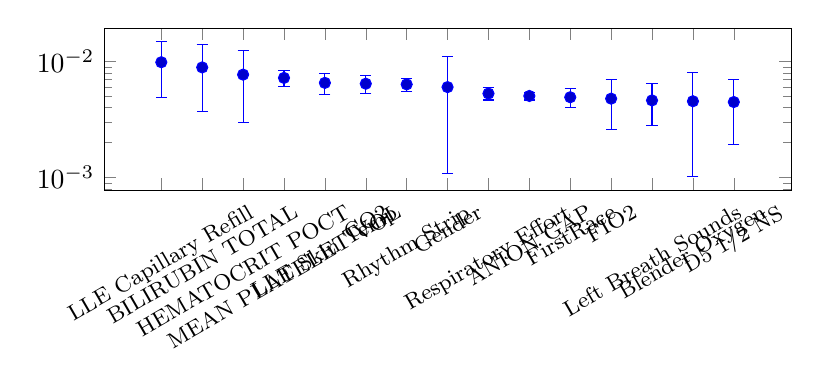
\begin{tikzpicture}
\begin{semilogyaxis} [
width=0.85\linewidth,
height=0.3\linewidth,
%log ticks with fixed point,
symbolic x coords={LLE Capillary Refill,BILIRUBIN TOTAL,HEMATOCRIT POCT,MEAN PLATELET VOL,LLE Skin Temp,CO2,Rhythm Strip,Gender,Respiratory Effort,ANION GAP,FirstRace,FIO2,Left Breath Sounds, Blender Oxygen,D5 1/2 NS},
xtick=data,
%ytick=data,
ymode=log, % Set y-axis to logarithmic scale
log basis y={10}, % Base 10 logarithm for the y-axis
xticklabel style = {font=\footnotesize, rotate=30},
]
\addplot+[only marks] plot[error bars/.cd, y dir=both, y explicit]
coordinates{
    (LLE Capillary Refill,0.00986033870379835) +- (0.0147661644336152,0.00495451297398151)
    (BILIRUBIN TOTAL,0.00889949693092115) +- (0.0126273414402402,0.00517165242160214) 
    (HEMATOCRIT POCT,0.00771484551610147) +- (0.0106733043693973,0.00475638666280566)
    (MEAN PLATELET VOL,0.00722791639121327) +- (0.0155413424057195,-0.00108550962329301)
    (LLE Skin Temp,0.00654834543779) +- (0.0117898135027299,0.00130687737285006)
    (CO2,0.00643982552509323) +- (0.0117188530496206,0.00116079800056584)
    (Rhythm Strip,0.0063570944708815) +- (0.0135076080519946,-0.00079341911023163)
    (Gender,0.0060215957123226) +- (0.007101505027428,0.00494168639721721)
    (Respiratory Effort,0.00529990635784179) +- (0.00995787056878017,0.000641942146903415)
    (ANION GAP,0.00505141865792101) +- (0.00971814564992059,0.000384691665921432)
    (FirstRace,0.00492530982150281) +- (0.00893863381241345,0.000911985830592171)
    (FIO2,0.00478955726231307) +- (0.00737036239483328,0.00220875212979286)
    (Left Breath Sounds,0.00462497034406318) +- (0.00745013982514881,0.00179980086297755)
    (Blender Oxygen,0.00454991688743892) +- (0.00556981498211942,0.00353001879275842)
    (D5 1/2 NS,0.00447869625451364) +- (0.00641773512494759,0.00253965738407969)
};
\end{semilogyaxis} 
\end{tikzpicture}
\caption{Feature importance analysis using feature permutation. Error bar indicates p95 high and p95 low.}
\label{fig:feat_important}
\vspace{-0.4cm}
\end{figure*}


\subsection{Experimental Results \& Discussion}
Table~\ref{tab:CHOA_main_exp} summarizes the performance of our proposed \modelname to ten baseline models on various evaluation metrics. 
Notably, \modelname achieves the highest Bal\_acc, F1, MCC, and AUPRC outperforming all baseline models by an average improvement of $10.71$, $9.45$, $9.55$, and $3.10$ separately. 
Additionally, \modelname ranks second in AUROC, with an average improvement of $11.57$ except for gMLP model. 
Among baseline models, XGBoost achieves the runner-up in Bal\_Acc, F1, and MCC, while gMLP achieves the second best in AUPRC and the highest AUROC. 
The slightly lower AUROC of \modelname compared to gMLP can be attributed to AUROC's emphasis on overall ranking separability, which does not necessarily translate into optimal classification decisions~\cite{tomavsev2021use}, particularly in highly imbalanced datasets. AUROC measures the ability of a model to distinguish between control and case classes across all possible classification thresholds. However, it averages performance across all thresholds and gives equal importance to the classification of both the majority (control) and minority (CA) classes. In highly imbalanced datasets such as the pediatric CA prediction scenario, this can be problematic because the model might perform well on predicting non-CA patients and still achieve a high AUROC, even if it struggles to correctly identify patients at high risk of CA. 
Furthermore, our results highlight the effectiveness of multimodal data fusion. Models based on tabular representations (i.e., those using last observed risk factors) generally achieve superior Bal\_Acc, F1, and MCC, whereas models leveraging time-series representations tend to perform better in AUPRC and AUROC. Integrating a tabular transformer to capture complex interactions among high-dimensional tabular risk factors and a pre-trained textual transformer to effectively model the dynamics of textualized time-series risk factors, \modelname delivers SOTA performance for CA risk prediction.

% bar chart
We further analyze XGBoost, gMLP, and \modelname in terms of Positive Predictive Value (PPV), Negative Predictive Value (NPV), Sensitivity, and Specificity, as shown in Figure~\ref{fig:bar_chart}, to align with clinical priorities. Overall, \modelname achieves the most balanced performance across all four metrics.
Specifically, \modelname demonstrates a slight advantage in both PPV and NPV, while gMLP exhibits high variance in PPV, as indicated by the wide error bars. Notably, \modelname attains the highest sensitivity, which is particularly crucial for screening CA, where missing cases can have severe consequences. At the same time, \modelname maintains competitive specificity, striking a careful balance between sensitivity and specificity—two metrics that often trade off inversely.
These observations further validate the limitations of AUROC as a sole evaluation metric, highlighting its tendency to be overly optimistic or misleading in highly imbalanced settings. While AUROC emphasizes ranking separability, it does not directly reflect clinical utility, whereas metrics like sensitivity and PPV better capture a model’s practical impact on early CA detection.


\subsection{Feature Importance Analysis}
We use permutation importance method~\cite{altmann2010permutation} to calculate the feature importance scores for our proposed perturbed copy of the data where this feature's values have been randomly shuffled across rows. We set number of different permutation shuffles as $5$, and the confidence level as $0.95$. Top 15 important features with $p\_value \leq 0.05$ are presented in Fig.~\ref{fig:feat_important}.
Our analysis reveals that key clinical indicators, such as capillary refill, total bilirubin level, and hematocrit, are among the most important predictors for pediatric cardiac arrest. 
Notably, factors related to hemodynamic stability and oxygenation/ventilation—including CO2 level on arterial blood gas, and FIO2,—also rank highly, emphasizing their critical role in patient monitoring. Furthermore, the inclusion of demographic factors such as sex and race highlights the multifactorial nature of cardiac arrest risk in the pediatric population.
Overall, this feature importance analysis not only identifies clinical risk factors but also uncovers novel predictors that may enhance early risk detection and guide future targeted interventions.

%\subsection{Ablation Study of Two Base Models}